\chapter{Análisis del problema}
\label{ch:analisis}
\paragraph*{}En este capítulo se presenta el análisis funcional del sistema desarrollado en el marco de este Trabajo de Fin de Grado. Al tratarse de una ampliación del dashboard desarrollado en un Trabajo de Fin de Grado previo, se mantienen sus características principales y se incorporan nuevas capacidades orientadas a mejorar el análisis, la comparación de técnicas y la interpretación de resultados.

\paragraph*{}El objetivo principal de esta ampliación es proporcionar una herramienta más flexible y completa para el estudio del abandono académico en el ámbito universitario. Para ello, se profundiza en los factores que influyen en este fenómeno mediante la incorporación de nuevas técnicas de análisis de supervivencia y funcionalidades complementarias.

\paragraph*{}El análisis parte de los requisitos funcionales, no funcionales y de información definidos en el capítulo anterior. A partir de ellos, se identifican los actores que interactúan con la aplicación y los casos de uso asociados a la ampliación propuesta. De este modo, las funcionalidades se describen desde la perspectiva del usuario y se representa su comportamiento mediante diagramas de casos de uso y diagramas de actividad, lo que facilita comprender el flujo de interacción entre los distintos componentes del sistema.



\section{Identificación de actores}
\paragraph*{}En esta primera fase de análisis del problema se mantienen los mismos actores principales que en el Trabajo de Fin de Grado anterior, ya que la aplicación está orientada al mismo tipo de público: profesorado, personal administrativo, alumnado o cualquier miembro interesado en utilizar estas técnicas a partir de los datos propuestos. Aunque la interacción principal recae sobre el usuario, también se considera el asistente de inteligencia artificial, encargado de procesar las consultas y generar respuestas o interpretaciones relacionadas con los resultados obtenidos.
\begin{itemize}
    \item \textbf{Usuario}: Representa a cualquier persona que utiliza la aplicación para cargar datos, ejecutar análisis de supervivencia, visualizar resultados, comparar modelos y exportar la información generada por el sistema.
    \item \textbf{Sistema de Inteligencia Artificial (IA)}: Actúa como un componente externo que interactúa con el usuario proporcionando explicaciones, sugerencias e interpretaciones de los resultados obtenidos. En esta nueva versión del sistema, este actor adquiere especial relevancia debido a las mejoras introducidas en la calidad y rapidez de las respuestas generadas.
\end{itemize}





\section{Identificación de casos de uso}
\paragraph*{}Dado que este Trabajo Fin de Grado supone una ampliación y mejora del dashboard desarrollado previamente, no resulta necesario incluir en la lista de casos de uso las funcionalidades ya implementadas en el proyecto anterior. Tras el análisis de los objetivos generales del proyecto y la elicitación de requisitos correspondiente, en esta fase se identifican y documentan las principales acciones que los actores previamente definidos pueden llevar a cabo sobre el sistema.
\begin{table}[H]
\centering
\small
\begin{tabularx}{\textwidth}{|p{1.1cm}|p{4.9cm}|X|}
\hline
\textbf{Id} & \textbf{Nombre} & \textbf{Descripción} \\ \hline

CU-1 & \raggedright Ejecutar modelo exponencial & 
Permite al usuario aplicar el modelo exponencial como técnica de análisis de supervivencia para estudiar el tiempo hasta el evento. \\ \hline

CU-2 & \raggedright Ejecutar modelo Weibull & 
Permite al usuario aplicar el modelo de Weibull para analizar el comportamiento del riesgo en función del tiempo mediante un enfoque paramétrico. \\ \hline

CU-3 & \raggedright Ejecutar Random Survival Forest & 
Permite al usuario aplicar el modelo Random Survival Forest para realizar análisis de supervivencia basados en técnicas de aprendizaje automático. \\ \hline

CU-4 & \raggedright Consultar comparación de técnicas & 
Permite al usuario acceder a una página específica del dashboard dedicada a la comparación de técnicas de análisis de supervivencia, mostrando una tabla comparativa, visualizaciones y un bloque explicativo automático. \\ \hline

CU-5 & \raggedright Exportar informes y resultados & 
Permite al usuario exportar resultados, gráficas y tablas generadas por el sistema en formato reutilizable para documentación o análisis posteriores. \\ \hline

CU-6 & \raggedright Cambiar idioma de la interfaz & 
Permite al usuario seleccionar y cambiar el idioma de la interfaz del sistema, facilitando su uso en distintos contextos lingüísticos. \\ \hline

CU-7 & \raggedright Analizar variables no binarias & 
Permite incorporar y analizar nuevas variables del conjunto de datos, incluyendo variables no binarias, ampliando las posibilidades de estudio del sistema. \\ \hline

CU-8 & \raggedright Mejorar interpretación con IA & 
Permite generar explicaciones más precisas, coherentes y rápidas mediante la mejora del sistema de inteligencia artificial integrado. \\ \hline

CU-9 & \raggedright Ampliar visualizaciones Cox y Test de Log-Rank & 
Permite generar nuevas visualizaciones asociadas a los modelos de regresión de Cox y Test de Log-Rank, mejorando la interpretación visual de los resultados. \\ \hline

\end{tabularx}
\caption{Identificación de casos de uso de la ampliación del sistema}
\label{tab:casos_uso_ampliacion}
\normalsize
\end{table}




\section{Diagrama de casos de uso}
Tras la identificación de los casos de uso y los actores, se procede a la creación del diagrama de casos de uso. Este diagrama, elaborado mediante la herramienta Visual Paradigm, representa de forma visual las funcionalidades del sistema y las interacciones que los actores pueden realizar sobre él.
Dicho diagrama se centra únicamente en los casos de uso asociados a la ampliación desarrollada, manteniendo implícitas las funcionalidades del sistema base. 


\begin{figure}[H]
    \centering
    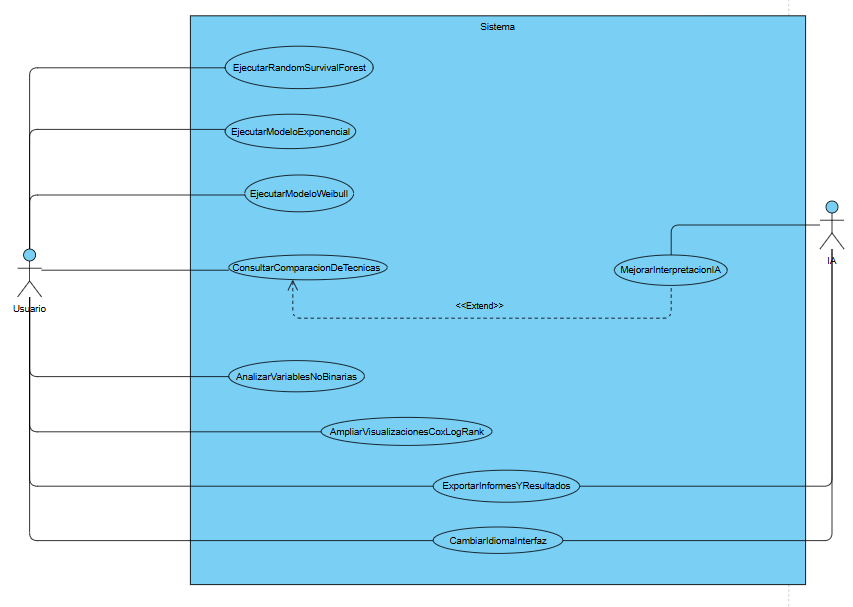
\includegraphics[width=1.0\textwidth]{Imagenes/diagrama_cu.png}
    \caption{Diagrama de casos de uso de la ampliación del sistema}
    \label{fig:Diagrama de casos de uso}
\end{figure}



\newpage
\section{Especificación de los casos de uso}
Una vez definidos los casos de uso, los actores del sistema y el diagrama general, se procede a la especificación de cada uno de ellos.
En dicha especificación se describe con detalle cómo funciona cada funcionalidad desde el punto de vista del usuario, incluyendo condiciones iniciales, resultados esperados y posibles errores. Además, se identifican los actores implicados en cada caso de uso.

    \subsection{CU-1: EjecutarModeloExponencial}
    \small
\begin{longtable}{|p{4cm}|p{10cm}|}
\caption{Especificación del CU-1: Ejecutar modelo exponencial}
\label{tab:esp_cu1}\\
\hline
\textbf{Id} & CU-1 \\ \hline
\textbf{Nombre} & EjecutarModeloExponencial \\ \hline

\textbf{Descripción} & 
Este caso de uso describe el proceso mediante el cual el usuario aplica el modelo exponencial como técnica de análisis de supervivencia, con el objetivo de estudiar el tiempo hasta la ocurrencia del evento analizado. \\ \hline

\textbf{Actor principal} & Usuario \\ \hline
\textbf{Actores secundarios} & Sistema \\ \hline

\textbf{Precondiciones} & 
\begin{itemize}
    \item El dataset debe haber sido cargado y preprocesado correctamente.
    \item El usuario debe haber accedido a la sección correspondiente al modelo exponencial.
\end{itemize} \\ \hline

\textbf{Flujo principal} & 
\begin{enumerate}
    \item El caso de uso comienza cuando el usuario accede al módulo de Análisis de Supervivencia y selecciona el botón ``Análisis Exponencial''.
    \item El sistema carga la vista del modelo exponencial y verifica que exista un dataset previamente cargado y preprocesado.
    \item El sistema detecta que hay un dataset disponible y calcula automáticamente el resultado del modelo.
    \item El sistema muestra en pantalla las salidas del módulo: tabla resumen, gráfica y comparativa de ajuste.
    \item El usuario decide una acción posterior:
    \begin{itemize}
        \item Pulsar botón ``Explicar''.
        \item Pulsar botón ``Exportar a PDF''.
        \item Pulsar botón ``Exportar informe combinado''.
    \end{itemize}
    \item El sistema ejecuta la acción seleccionada y muestra la confirmación o resultado correspondiente.
\end{enumerate} \\ \hline

\textbf{Postcondiciones} & 
El análisis mediante el modelo exponencial queda completado y los resultados quedan disponibles para su visualización, comparación o exportación posterior. \\ \hline

\textbf{Flujos alternativos} & 
\textbf{FA1 (Ejecución del modelo):} El sistema no puede ejecutar el modelo debido a datos insuficientes o incompatibles. El sistema muestra un mensaje de error indicando la imposibilidad de realizar el análisis. \\ \hline

\end{longtable}

\newpage
    \small
    \subsection{CU-2: EjecutarModeloWeibull}
    \begin{longtable}{|p{4cm}|p{10cm}|}
\caption{Especificación del CU-2: Ejecutar modelo Weibull}
\label{tab:esp_cu2}\\
\hline
\textbf{Id} & CU-2 \\ \hline
\textbf{Nombre} & EjecutarModeloWeibull \\ \hline

\textbf{Descripción} & 
Este caso de uso describe el proceso mediante el cual el usuario aplica el modelo de Weibull como técnica de análisis de supervivencia, permitiendo analizar el comportamiento del riesgo a lo largo del tiempo mediante un enfoque paramétrico. \\ \hline

\textbf{Actor principal} & Usuario \\ \hline
\textbf{Actores secundarios} & Sistema \\ \hline

\textbf{Precondiciones} & 
\begin{itemize}
    \item El dataset debe haber sido cargado y preprocesado correctamente.
    \item El usuario debe haber accedido a la sección correspondiente al modelo de Weibull.
\end{itemize} \\ \hline

\textbf{Flujo principal} & 
\begin{enumerate}
    \item El caso de uso comienza cuando el usuario accede al módulo de Análisis de Supervivencia y selecciona el botón ``Análisis Weibull''.
    \item El sistema carga la vista del modelo de Weibull y verifica que exista un dataset previamente cargado y preprocesado.
    \item El sistema detecta que hay un dataset disponible y calcula automáticamente el resultado del modelo.
    \item El sistema muestra en pantalla las salidas del módulo: tabla resumen, gráfica y comparativa de ajuste.
    \item El usuario decide una acción posterior:
    \begin{itemize}
        \item Pulsar botón ``Explicar''.
        \item Pulsar botón ``Exportar a PDF''.
        \item Pulsar botón ``Exportar informe combinado''.
    \end{itemize}
    \item El sistema ejecuta la acción seleccionada y muestra la confirmación o resultado correspondiente.
\end{enumerate} \\ \hline

\textbf{Postcondiciones} & 
Los resultados quedan disponibles para su visualización, comparación o exportación. \\ \hline

\textbf{Flujos alternativos} & 
\textbf{FA1 (Ejecución del modelo):} El sistema detecta un error en los datos o parámetros seleccionados. El sistema muestra un mensaje indicando la imposibilidad de ejecutar el modelo. \\ \hline

\end{longtable}
\newpage


    \subsection{CU-3: EjecutarRandomSurvivalForest}
        \small
\begin{longtable}{|p{4cm}|p{10cm}|}
\caption{Especificación del CU-3: Ejecutar Random Survival Forest}
\label{tab:esp_cu3}\\
\hline
\textbf{Id} & CU-3 \\ \hline
\textbf{Nombre} & EjecutarRandomSurvivalForest \\ \hline

\textbf{Descripción} & 
Este caso de uso describe el proceso mediante el cual el usuario aplica el modelo Random Survival Forest para realizar análisis de supervivencia mediante técnicas de aprendizaje automático. \\ \hline

\textbf{Actor principal} & Usuario \\ \hline
\textbf{Actores secundarios} & Sistema \\ \hline

\textbf{Precondiciones} & 
\begin{itemize}
    \item El dataset debe haber sido cargado y preprocesado correctamente.
    \item El usuario debe haber accedido a la sección correspondiente a Random Survival Forest.
\end{itemize} \\ \hline

\textbf{Flujo principal} & 
\begin{enumerate}
    \item El caso de uso comienza cuando el usuario accede al módulo de Análisis de Supervivencia y selecciona el botón ``Random Survival Forest''.
    
    \item El sistema detecta la ruta correspondiente y ejecuta automáticamente el análisis utilizando el dataset en sesión.
    
    \item El sistema muestra en pantalla los resultados del modelo, incluyendo:
    \begin{itemize}
        \item Tabla resumen del modelo.
        \item Gráfica de curvas de supervivencia estimadas por niveles de riesgo.
        \item Gráfica de importancia de variables.
    \end{itemize}
    
    \item El sistema muestra el panel de simulación de perfil con valores por defecto (género, discapacidad, edad, educación, créditos) junto con una primera estimación del perfil.
    
    \item El usuario revisa los resultados obtenidos y, si lo desea, modifica los valores del perfil.
    
    \item El usuario puede pulsar el botón ``Simular perfil'' para recalcular y visualizar el detalle del perfil, incluyendo curva de supervivencia, interpretación y métricas asociadas.
    
    \item El usuario decide una acción posterior:
    \begin{itemize}
        \item Pulsar el botón ``Explicar''.
        \item Pulsar el botón ``Exportar a PDF''.
    \end{itemize}
    
    \item El sistema ejecuta la acción seleccionada y muestra la confirmación o resultado correspondiente.
\end{enumerate} \\ \hline

\textbf{Postcondiciones} & 
Los resultados quedan disponibles para su visualización, comparación o exportación. \\ \hline

\textbf{Flujos alternativos} & 
\textbf{FA1 (Ejecución del modelo):} El sistema no puede completar el entrenamiento o ejecución del modelo. El sistema informa al usuario mediante un mensaje de error. \\ \hline

\end{longtable}
\newpage


    \subsection{CU-4: ConsultarComparacionDeTecnicas}

\begin{longtable}{|p{4cm}|p{10cm}|}
\caption{Especificación del CU-4: Consultar comparación de técnicas}
\label{tab:esp_cu4}\\
\hline
\textbf{Id} & CU-4 \\ \hline
\textbf{Nombre} & ConsultarComparacionDeTecnicas \\ \hline

\textbf{Descripción} & 
Este caso de uso describe el proceso mediante el cual el usuario accede a una página específica del dashboard dedicada a la comparación de técnicas de análisis de supervivencia, con el objetivo de consultar información comparativa entre los distintos métodos implementados en el sistema. \\ \hline

\textbf{Actor principal} & Usuario \\ \hline
\textbf{Actores secundarios} & Sistema de Inteligencia Artificial (IA) \\ \hline

\textbf{Precondiciones} & 
\begin{itemize}
    \item El usuario debe haber accedido previamente a la sección ``Análisis de supervivencia'' del dashboard.
    \item La página ``Comparación de técnicas'' debe estar integrada en el sistema de rutas de la aplicación.
    \item La opción de acceso a esta funcionalidad debe estar disponible en el menú superior únicamente cuando el usuario se encuentre en la sección correspondiente.
\end{itemize} \\ \hline

\textbf{Flujo principal} & 
\begin{enumerate}
    \item El caso de uso comienza cuando el usuario accede a la página ``Comparación de técnicas''.
    
    \item El sistema valida que exista un dataset disponible en la sesión.
    
    \item El sistema carga automáticamente una tabla comparativa de técnicas que incluye información como el tipo de modelo, hipótesis, ventajas, limitaciones y contexto de uso recomendado.
    
    \item El sistema genera una visualización comparativa en forma de gráfico de barras, mostrando puntuaciones orientativas (capacidad predictiva, interpretabilidad y flexibilidad en una escala de 0 a 5).
    
    \item El sistema genera un bloque explicativo textual mediante el módulo de inteligencia artificial, en el que se resumen las principales diferencias entre técnicas y se propone una estrategia metodológica de uso.
    
    \item El usuario consulta la información mostrada y la utiliza como apoyo para el análisis e interpretación de los resultados.
\end{enumerate} \\ \hline

\textbf{Postcondiciones} & 
La página de comparación de técnicas queda cargada correctamente y la información comparativa permanece disponible para su consulta, interpretación o posible exportación posterior. \\ \hline

\textbf{Flujos alternativos} & 
\begin{itemize}
    \item \textbf{FA1 (Carga de la página):} el sistema no puede cargar correctamente la página de comparación. En ese caso, muestra un mensaje de error al usuario indicando la imposibilidad de acceder a dicha funcionalidad.
    
    \item \textbf{FA2 (Generación de visualización comparativa):} no es posible generar el gráfico comparativo debido a la falta de datos o a incompatibilidades entre las técnicas. El sistema mantiene visible la tabla comparativa y el bloque explicativo automático, pero omite la visualización gráfica.
    
    \item \textbf{FA3 (Generación del bloque explicativo):} el sistema no puede generar el texto explicativo automático. El sistema mantiene visible la tabla comparativa y, en su caso, la visualización gráfica, mostrando un aviso al usuario.
\end{itemize} \\ \hline

\end{longtable}
    \newpage
    \subsection{CU-5: ExportarInformesYResultados}
    
\begin{longtable}{|p{4cm}|p{10cm}|}
\caption{Especificación del CU-5: Exportar informes y resultados}
\label{tab:esp_cu5}\\
\hline
\textbf{Id} & CU-5 \\ \hline
\textbf{Nombre} & ExportarInformesYResultados \\ \hline

\textbf{Descripción} & 
Este caso de uso describe el proceso mediante el cual el usuario exporta los resultados, gráficas y tablas generadas por el sistema en un formato reutilizable. \\ \hline

\textbf{Actor principal} & Usuario \\ \hline
\textbf{Actores secundarios} & Sistema \\ \hline

\textbf{Precondiciones} & 
\begin{itemize}
    \item Deben existir resultados generados previamente en el sistema.
    \item El usuario debe haber accedido a la funcionalidad de exportación.
\end{itemize} \\ \hline

\textbf{Flujo principal} & 
\begin{enumerate}
    \item El caso de uso comienza cuando el usuario pulsa el botón ``Exportar a PDF'' del módulo correspondiente.
    
    \item El sistema abre un modal de exportación.
    
    \item El usuario introduce, de forma opcional, el nombre del archivo y selecciona el contenido a incluir en el informe.
    
    \item El usuario confirma la operación pulsando ``Descargar PDF''.
    
    \item El sistema valida que existan datos o resultados suficientes para realizar la exportación.
    
    \item El sistema genera el informe en formato PDF con los bloques seleccionados (resumen, tabla, gráfica e interpretación, según el módulo).
    
    \item El sistema entrega el archivo generado para su descarga.
\end{enumerate} \\ \hline

\textbf{Postcondiciones} & 
El archivo de resultados queda generado correctamente y puede ser utilizado en documentación o análisis posteriores. \\ \hline

\textbf{Flujos alternativos} & 
\textbf{FA1 (Generación del archivo):} El sistema no puede generar el archivo. El sistema muestra un mensaje de error al usuario. \\ \hline

\end{longtable}
    \newpage
    
    \subsection{CU-6: CambiarIdiomaInterfaz}
\begin{longtable}{|p{4cm}|p{10cm}|}
\caption{Especificación del CU-6: Cambiar idioma de la interfaz}
\label{tab:esp_cu6}\\
\hline
\textbf{Id} & CU-6 \\ \hline
\textbf{Nombre} & CambiarIdiomaInterfaz \\ \hline

\textbf{Descripción} & 
Este caso de uso describe el proceso mediante el cual el usuario cambia el idioma de la interfaz del sistema. \\ \hline

\textbf{Actor principal} & Usuario \\ \hline
\textbf{Actores secundarios} & Sistema \\ \hline

\textbf{Precondiciones} & 
\begin{itemize}
    \item El sistema debe estar en ejecución.
    \item Deben existir varios idiomas disponibles.
\end{itemize} \\ \hline

\textbf{Flujo principal} & 
\begin{enumerate}
    \item El caso de uso comienza cuando el usuario accede al selector de idioma de la barra de navegación.
    
    \item El sistema muestra los idiomas disponibles.
    
    \item El usuario selecciona el idioma deseado.
    
    \item El sistema procesa la selección y recarga los textos visibles de la interfaz en el idioma seleccionado.
    
    \item Finalmente, la interfaz se muestra completamente actualizada en el idioma elegido.
\end{enumerate} \\ \hline

\textbf{Postcondiciones} & 
El idioma de la interfaz queda actualizado correctamente. \\ \hline

\textbf{Flujos alternativos} & 
\textbf{FA1 (Cambio de idioma):} El sistema no puede aplicar el idioma seleccionado. El sistema mantiene el idioma anterior y muestra un mensaje de aviso al usuario. \\ \hline

\end{longtable}
    \newpage
    \subsection{CU-7: AnalizarVariablesNoBinarias}
\begin{longtable}{|p{4cm}|p{10cm}|}
\caption{Especificación del CU-7: Analizar variables no binarias}
\label{tab:esp_cu7}\\
\hline
\textbf{Id} & CU-7 \\ \hline
\textbf{Nombre} & AnalizarVariablesNoBinarias \\ \hline

\textbf{Descripción} & 
Este caso de uso describe el proceso mediante el cual el usuario incorpora y analiza nuevas variables del conjunto de datos, incluyendo variables no binarias. \\ \hline

\textbf{Actor principal} & Usuario \\ \hline
\textbf{Actores secundarios} & Sistema \\ \hline

\textbf{Precondiciones} & 
\begin{itemize}
    \item El dataset debe haber sido cargado correctamente.
    \item Deben existir variables adicionales o no binarias en el conjunto de datos.
\end{itemize} \\ \hline

\textbf{Flujo principal} & 
\begin{enumerate}
    \item El caso de uso comienza cuando el usuario carga un archivo CSV y pulsa la opción ``Preprocesar CSV''.
    
    \item El sistema valida la estructura del dataset y conserva las variables no binarias soportadas por el pipeline.
    
    \item El usuario accede al módulo de análisis de covariables o supervivencia y selecciona una variable no binaria disponible.
    
    \item El sistema transforma la variable según la técnica aplicada (por ejemplo, agrupación por categorías o discretización por cuantiles en variables como créditos).
    
    \item El sistema ejecuta el análisis correspondiente utilizando las variables seleccionadas.
    
    \item El sistema muestra en pantalla los resultados actualizados, incluyendo tablas, métricas y representaciones gráficas.
    
    \item El usuario consulta los resultados y los utiliza para interpretar el efecto de las variables analizadas.
\end{enumerate} \\ \hline

\textbf{Postcondiciones} & 
Las nuevas variables quedan integradas en el análisis y los resultados quedan disponibles para su interpretación. \\ \hline

\textbf{Flujos alternativos} & 
\textbf{FA1 (Validación de variables):} El sistema detecta que alguna variable no es compatible con el análisis seleccionado. El sistema informa al usuario mediante un mensaje de error. \\ \hline

\end{longtable}
    \newpage
    \subsection{CU-8: MejorarInterpretacionIA}
\begin{longtable}{|p{4cm}|p{10cm}|}
\caption{Especificación del CU-8: Mejorar interpretación mediante IA}
\label{tab:esp_cu8}\\
\hline
\textbf{Id} & CU-8 \\ \hline
\textbf{Nombre} & MejorarInterpretacionIA \\ \hline

\textbf{Descripción} & 
Este caso de uso describe el proceso mediante el cual el sistema genera explicaciones más precisas, coherentes y rápidas mediante una mejora del módulo de inteligencia artificial. \\ \hline

\textbf{Actor principal} & Sistema de Inteligencia Artificial (IA) \\ \hline
\textbf{Actores secundarios} & Usuario \\ \hline

\textbf{Precondiciones} & 
\begin{itemize}
    \item Deben existir resultados generados previamente en el sistema.
    \item El módulo de inteligencia artificial debe estar disponible.
\end{itemize} \\ \hline

\textbf{Flujo principal} & 
\begin{enumerate}
    \item El caso de uso comienza cuando el usuario solicita una interpretación de los resultados obtenidos.
    
    \item El sistema recopila la información relevante del análisis ejecutado.
    
    \item El sistema envía dicha información al módulo de inteligencia artificial.
    
    \item El módulo de inteligencia artificial procesa los datos y genera una explicación.
    
    \item El sistema recibe la respuesta generada y la presenta en la interfaz para su consulta por parte del usuario.
\end{enumerate} \\ \hline

\textbf{Postcondiciones} & 
La explicación generada queda disponible para el usuario, facilitando la interpretación de los resultados. \\ \hline

\textbf{Flujos alternativos} & 
\textbf{FA1 (Generación de respuesta):} La inteligencia artificial no puede generar una respuesta adecuada. El sistema muestra un mensaje de error al usuario. \\ \hline

\end{longtable}

    \newpage
    \subsection{CU-9: AmpliarVisualizacionesCoxTestLogRank}
    \begin{longtable}{|p{4cm}|p{10cm}|}
\caption{Especificación del CU-9: Ampliar visualizaciones Cox y Test de Log-Rank}
\label{tab:esp_cu9}\\
\hline
\textbf{Id} & CU-9 \\ \hline
\textbf{Nombre} & AmpliarVisualizacionesCoxTestLogRank \\ \hline

\textbf{Descripción} & 
Este caso de uso describe el proceso mediante el cual el sistema genera nuevas visualizaciones asociadas a los modelos de regresión de Cox y Test de Log-Rank. \\ \hline

\textbf{Actor principal} & Usuario \\ \hline
\textbf{Actores secundarios} & Sistema \\ \hline

\textbf{Precondiciones} & 
\begin{itemize}
    \item Deben haberse ejecutado previamente análisis mediante regresión de Cox o Test de Log-Rank.
    \item Los resultados correspondientes deben estar disponibles en el sistema.
\end{itemize} \\ \hline

\textbf{Flujo principal} & 
\begin{enumerate}
    \item El caso de uso comienza cuando el usuario accede al módulo de análisis de supervivencia y selecciona ``Regresión de Cox'' o ``Test de Log-Rank''.
    
    \item El sistema muestra las opciones de visualización disponibles.
    
    \item El usuario selecciona la visualización deseada.
    
    \item El sistema obtiene los resultados del análisis correspondientes a la configuración activa.
    
    \item El sistema procesa la información y genera la representación gráfica solicitada.
    
    \item El sistema muestra la visualización en pantalla para su consulta por parte del usuario.
\end{enumerate} \\ \hline

\textbf{Postcondiciones} & 
La visualización queda generada correctamente y disponible para su interpretación o exportación. \\ \hline

\textbf{Flujos alternativos} & 
\textbf{FA1 (Disponibilidad de datos):} No existen resultados previos de Cox o Test de Log-Rank. El sistema informa al usuario de que debe ejecutar previamente dichos análisis. \\ \hline

\end{longtable}


\section{Matriz de trazabilidad}
La siguiente matriz muestra la relación entre los Requisitos Funcionales (RF) definidos 
para el sistema y los Casos de Uso (CU) que los implementan. De este modo se 
garantiza la cobertura de todos los requisitos dentro del diseño y desarrollo de la 
aplicación. 
\begin{table}[H]
\centering
\small
\begin{tabular}{|c|c|c|c|c|c|c|c|c|c|}
\hline
\textbf{Req} & \textbf{CU-1} & \textbf{CU-2} & \textbf{CU-3} & \textbf{CU-4} & \textbf{CU-5} & \textbf{CU-6} & \textbf{CU-7} & \textbf{CU-8} & \textbf{CU-9} \\ \hline

RF1  &  &  &  & X &  &  &  & X &  \\ \hline
RF2  &  &  &  &  &  & X &  &  &  \\ \hline
RF3  &  &  &  &  &  &  & X &  &  \\ \hline
RF4  &  &  &  &  &  &  & X &  &  \\ \hline
RF5  &  &  &  &  &  &  &  &  & X \\ \hline
RF6  & X & X & X &  &  &  &  &  &  \\ \hline
RF7  & X &  &  &  &  &  &  &  &  \\ \hline
RF8  &  & X &  &  &  &  &  &  &  \\ \hline
RF9  &  &  & X &  &  &  &  &  &  \\ \hline
RF10 &  &  &  & X &  &  &  &  &  \\ \hline
RF11 &  &  &  &  &  &  &  & X &  \\ \hline
RF12 &  &  &  &  &  &  &  & X &  \\ \hline
RF13 & X & X & X &  & X &  &  &  &  \\ \hline

\end{tabular}
\caption{Matriz de trazabilidad entre requisitos funcionales y casos de uso}
\label{tab:trazabilidad}
\normalsize
\end{table}
\paragraph*{}Como puede observarse en la matriz, todos los requisitos funcionales definidos para la ampliación del sistema quedan cubiertos por al menos un caso de uso. Esto permite comprobar que no existen requisitos funcionales aislados sin representación en el análisis. En el caso concreto de RF13, la trazabilidad se asocia al caso de uso general de exportación y también a los modelos Exponencial, Weibull y Random Survival Forest, ya que estas vistas incorporan acciones específicas para generar informes o exportar resultados. Asimismo, cada caso de uso se relaciona con una o varias necesidades concretas del sistema, lo que facilita mantener la trazabilidad entre los objetivos planteados, los requisitos especificados y las funcionalidades que finalmente se desarrollan en la aplicación.


\newpage


\section{Diagramas de actividad}

\subsection{CU-1: EjecutarModeloExponencial}
\begin{figure}[H]
    \centering
    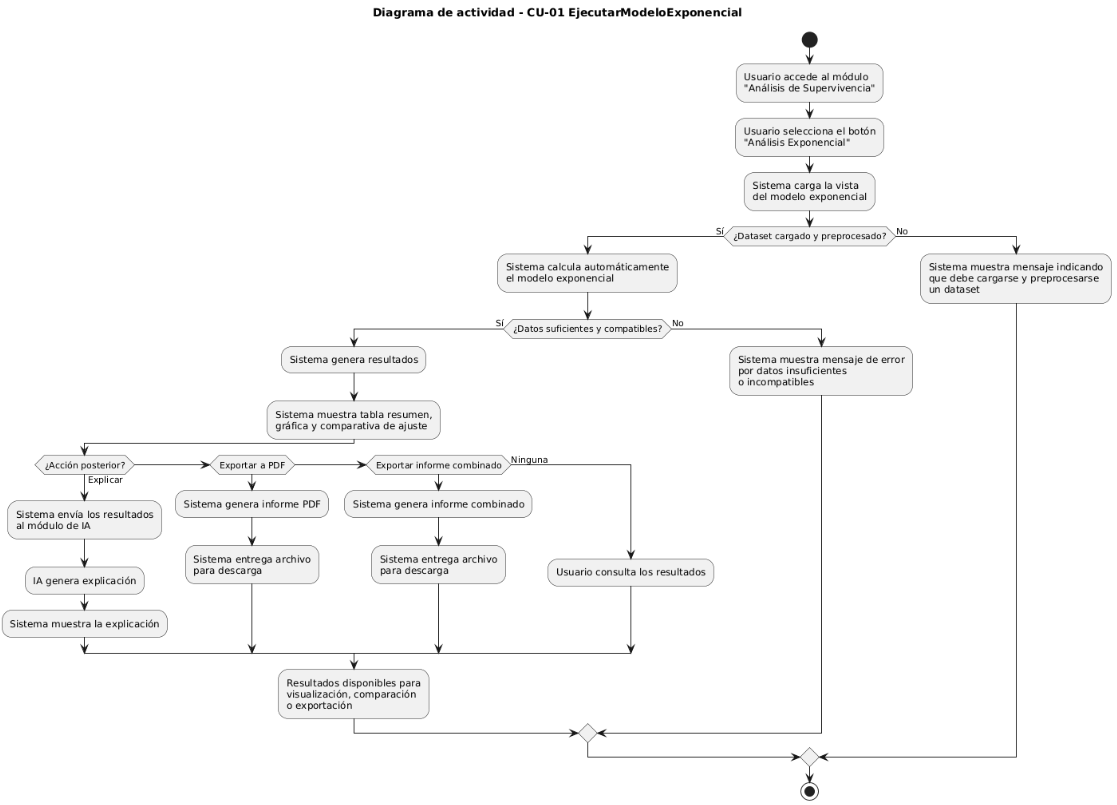
\includegraphics[width=\textwidth]{Imagenes/act_cu1.png}
    \caption{Diagrama de actividad del CU-1: EjecutarModeloExponencial}
    \label{fig:act_cu1}
\end{figure}


\subsection{CU-2: EjecutarModeloWeibull}
\begin{figure}[H]
    \centering
    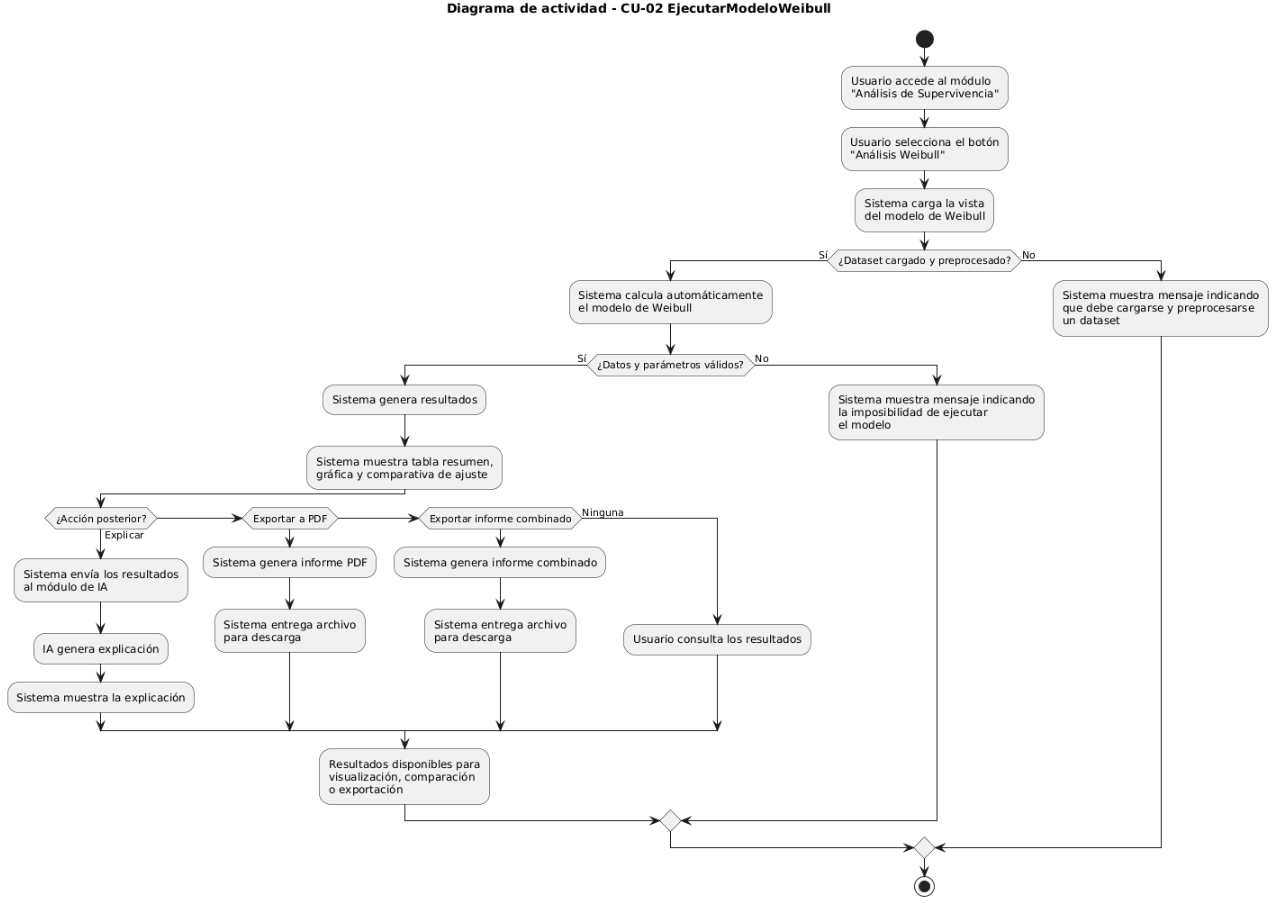
\includegraphics[width=\textwidth]{Imagenes/act_cu2.png}
    \caption{Diagrama de actividad del CU-2: EjecutarModeloWeibull}
    \label{fig:act_cu2}
\end{figure}


\subsection{CU-3: EjecutarRandomSurvivalForest}
\begin{figure}[H]
    \centering
    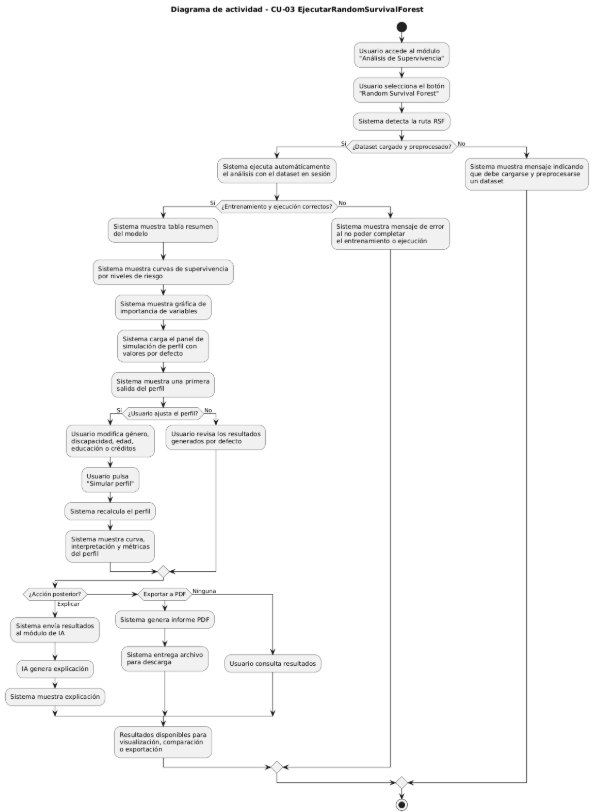
\includegraphics[width=0.9\textwidth]{Imagenes/act_cu3.png}
    \caption{Diagrama de actividad del CU-3: EjecutarRandomSurvivalForest}
    \label{fig:act_cu3}
\end{figure}


\subsection{CU-4: ConsultarComparacionDeTecnicas}
\begin{figure}[H]
    \centering
    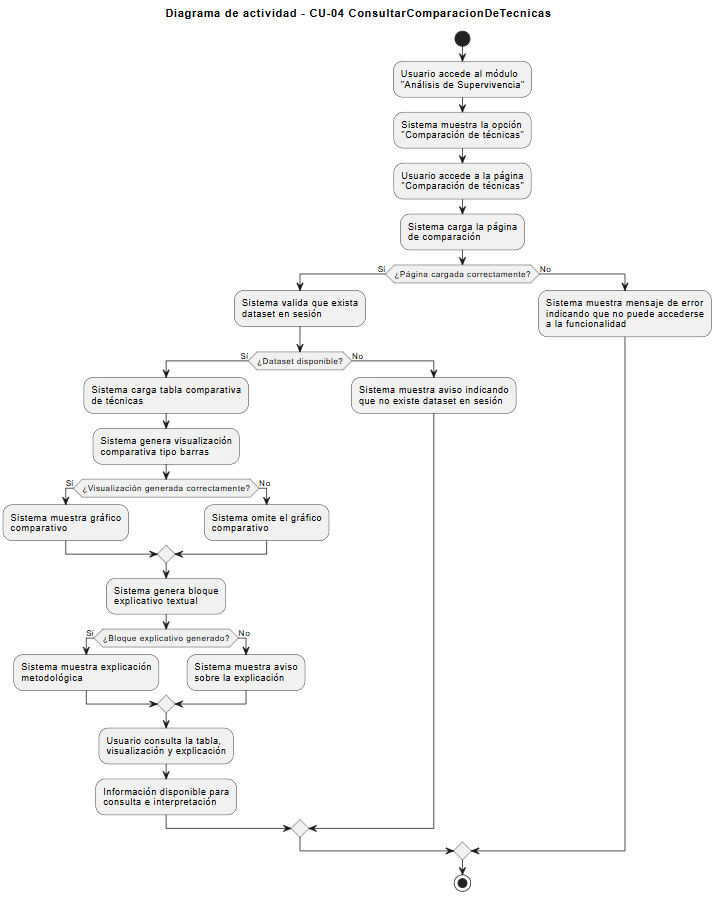
\includegraphics[width=\textwidth]{Imagenes/act_cu4.png}
    \caption{Diagrama de actividad del CU-4: ConsultarComparacionDeTecnicas}
    \label{fig:act_cu4}
\end{figure}

\subsection{CU-5: ExportarInformesYResultados}
\begin{figure}[H]
    \centering
    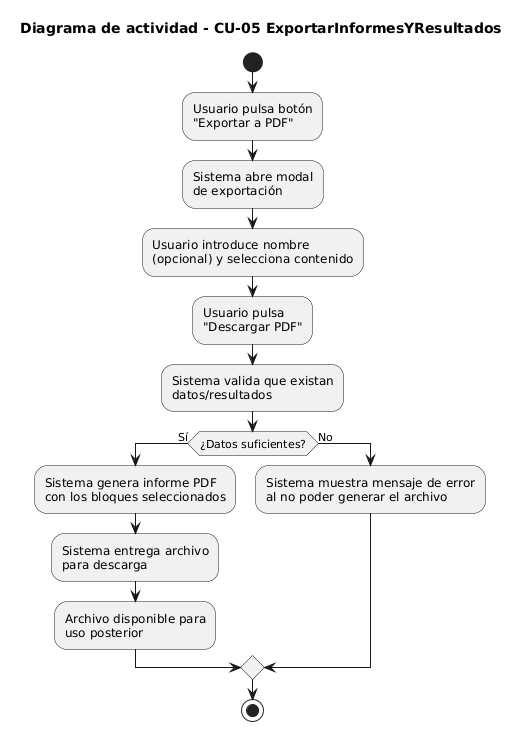
\includegraphics[width=0.8\textwidth]{Imagenes/act_cu5.png}
    \caption{Diagrama de actividad del CU-5: ExportarInformesYResultados}
    \label{fig:act_cu5}
\end{figure}


\subsection{CU-6: CambiarIdiomaInterfaz}
\begin{figure}[H]
    \centering
    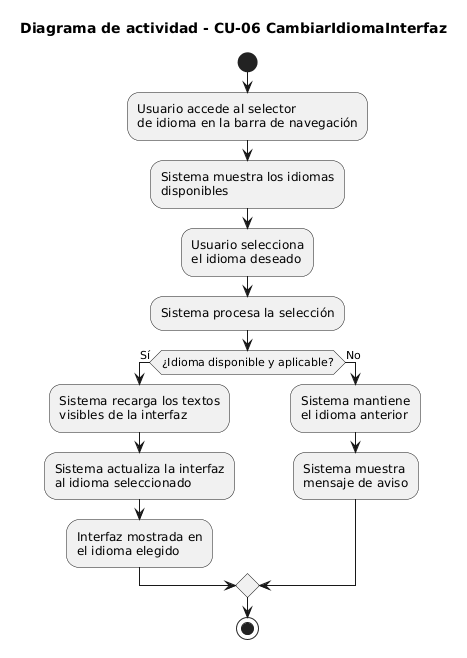
\includegraphics[width=0.85\textwidth]{Imagenes/act_cu6.png}
    \caption{Diagrama de actividad del CU-6: CambiarIdiomaInterfaz}
    \label{fig:act_cu6}
\end{figure}

\subsection{CU-7: AnalizarVariablesNoBinarias}
\begin{figure}[H]
    \centering
    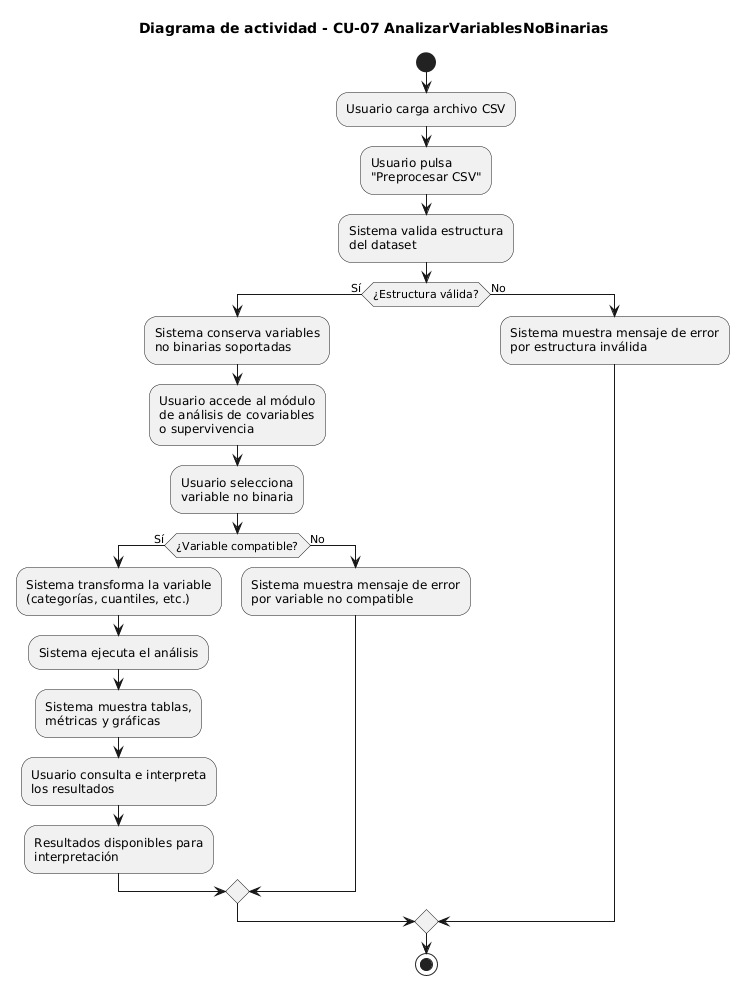
\includegraphics[width=0.9\textwidth]{Imagenes/act_cu7.png}
    \caption{Diagrama de actividad del CU-7: AnalizarVariablesNoBinarias}
    \label{fig:act_cu7}
\end{figure}

\subsection{CU-8: MejorarInterpretacionIA}
\begin{figure}[H]
    \centering
    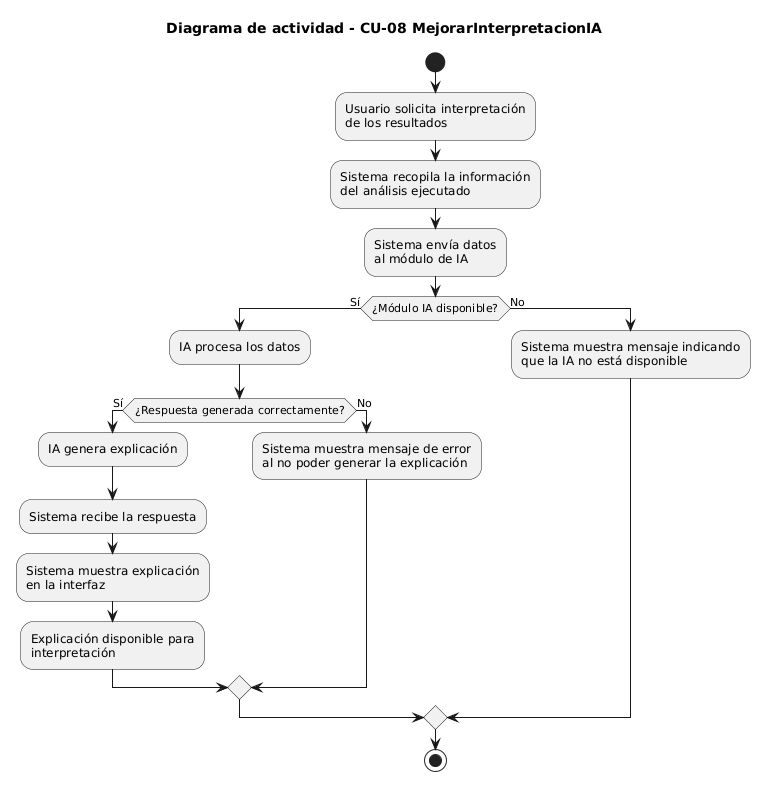
\includegraphics[width=\textwidth]{Imagenes/act_cu8.png}
    \caption{Diagrama de actividad del CU-8: MejorarInterpretacionIA}
    \label{fig:act_cu8}
\end{figure}

\subsection{CU-9: AmpliarVisualizacionesCoxTestLogRank}
\begin{figure}[H]
    \centering
    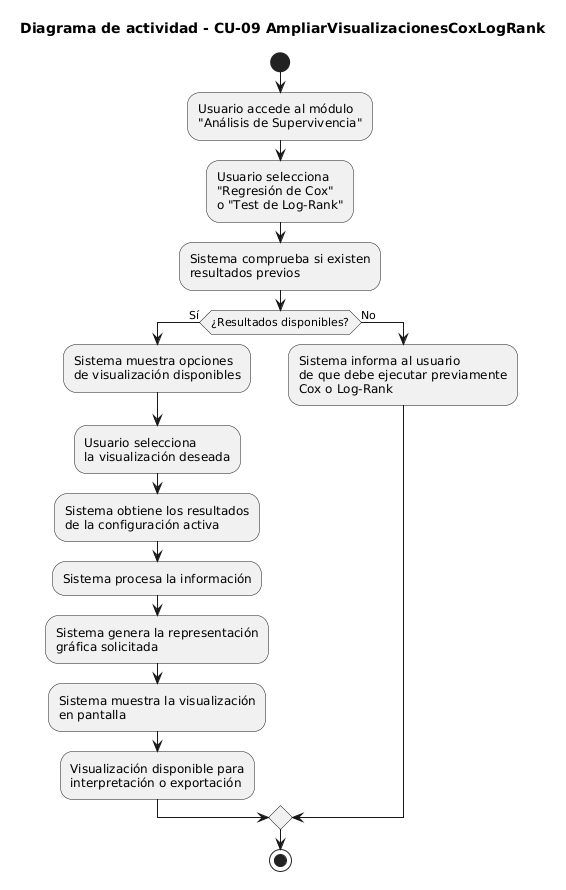
\includegraphics[width=0.8\textwidth]{Imagenes/act_cu9.png}
    \caption{Diagrama de actividad del CU-9: AmpliarVisualizacionesCoxTestLogRank}
    \label{fig:act_cu9}
\end{figure}
